\chapter{Systems of Equations}

A system of equations means having more than one relationship representing the system of interest. We will study systems composed of 2 linear equations and 2 unknowns. Systems with more equations and more variables are possible and will be covered in future courses. Three approaches to solve systems of equations will be covered here:
\begin{itemize}
	\item substitution
	\item elimination
	\item graphing
\end{itemize}

You could be asked to solve a system of 2 equations with 2 unknowns where one equation is linear and the other is not. Also you could be asked to solve a system of two nonlinear
equations although these will be restricted to very straightforward examples. It helps if you can visualise
the shape of the 2 equations so that the meaning of the solution is clear in your mind. An example will come later in the course when we find the area between two curves by integration where the intersection of these two curves represents the solution to a system of two equations.

We know that linear equations in two variables are represented by straight lines. Straight
lines will always intersect unless they are parallel. The coordinates of the point of intersection of the straight
lines is called the solution. you could use a graphical method or one of the two algebraic methods (substitution
or elimination) to find the solution. Parallel lines will never meet so will have no solution. Sometimes
the two equations will be two different representations of the same line so we say that in this case the system has an infinite number of solutions. 

\section{Solution by Substitution}
\subsubsection{Example 1}
Consider the system of equations
\begin{align}x^{2} +y^{2} &  = 25 \tag{1} \\
3 y +x &  = 15 \tag{2}\end{align}

We rearrange equation 2 and substitute into equation 1
\begin{align*}x &  =  15 -3 y \\
	&  =  3 \left (5 -y\right ) \\
	\text{so }\quad x^{2} &  =  9 \left (25 -10 y +y^{2}\right ) \\
	&  =  9 y^{2} -90 y +225\end{align*}

Equation 1 becomes
\begin{align*}9 y^{2} -90 y +225 +y^{2} &  =  25 \\
	10 y^{2} -90 y +200 &  =  0 \\
	y^{2} -9 y +20 &  = 0 \\
	\left (y -5\right ) \left (y -4\right ) &  =  0 \\
	\text{Either }\quad y -5 &  =  0\quad\text{ so }\quad y =5 \\
	\text{or }\quad y -4 &  =  0\quad\text{ so }\quad y =4\end{align*}

Back-substitute into equation 2 

When $y =5$, $3 y +x =15 \leadsto 15 +x =15 \Longleftrightarrow x =0$. This means $\left (0 ,5\right )$ is a solution. 

When $y =4$, $3 y +x =15 \leadsto 12 +x =15 \Longleftrightarrow x =3$. This means $\left (3 ,4\right )$ is a solution. 

\subsubsection{Example 2}
Now consider the system of equations
\begin{align}x^{2} +y^{2} &  =  25 \tag{3} \\
4 y +3 x &  =  25 \tag{4}\end{align}

Proceeding in the same way
\begin{align*}3 x &  =  25 -4 y \\
	\text{So\ \ \ }9 x^{2} &  =  \left (25 -4 y\right )^{2} \\
	&  =  625 -200 y +16 y^{2} \\
	&  =  16 y^{2} -200 y +625\end{align*}

From equation 3\qquad (Multiply equation 3 by 9)
\begin{align*}9 x^{2} +9 y^{2} &  =  225 \\
	\text{So}\quad 16 y^{2} -200 y +625 +9 y^{2} &  = 225\text{\ }{\tiny 9}{\tiny x}^{{\small 2}}\text{} \\
	\text{or}\quad 25 y^{2} -200 y +625 -225 &  =  0 \\
	25 y^{2} -200 y +400 &  =  0\text{\ \ } \\
	\text{or} \quad y^{2} -8 y +16 &  = 0 \\
	\left (y -4\right ) \left (y -4\right ) &  = 0 \\
	\text{So}\quad y &  =  4\end{align*}

Back substitute into equation 4 

When $y =4$, $4 y +3 x =25 \leadsto 16 +3 x =25 \Longleftrightarrow x =3$. This means $\left (3 ,4\right )$ is a solution. The
line cuts the circle in only one point. This means the line touches the circle. The
line is a tangent to the circle. You may verify by graphing the functions.

\subsection{Exercise}
\begin{enumerate}
	\item How can we invent a line parallel to $4 y +3 x =25$ that cuts the circle (in two points)? 
	
	\item How can we invent a line parallel
	to $4 y +3 x =25$ that misses the circle (cuts the circle in no points)? \end{enumerate}


Solution:
\ There are an infinite number of possibilities one such line that will cut the circle in two points is $4 y +3 x =24$, and a line that will miss the circle is $4 y +3 x =26$. 

\section{Solution by Elimination}
Refer to lecture notes.
\section{Solution by Graphing}
Refer to lecture notes.
\section{Infinite Solutions}
\emph{Example of a System with an Infinite Number of Solutions}\\
If you start with a linear equation such as $y -2 x =3$ and multiply each term by a constant you will get an equivalent equation. If you multiply the equation by another number you
will get a further equivalent equation.
\begin{equation*}y -2 x =3
\end{equation*}

Multiply by $2$
\begin{equation*}2 y -4 x =6
\end{equation*}

Multiply by $ -3$
\begin{align*} -3 y +6 x &  = &  -9 \\
\text{or}6 x -3 y +9 &  = & 0\end{align*}

We know these are both just different ways of writing the original equation $y -2 x =3$ or $y =2 x +3$. To say the system has an infinite number of solutions we are really saying every point
on $y =2 x +3$ is a solution. 


%
%We have a further way to represent these equations which we will introduce here. It
%is called the \emph{parametric} form of a straight line. In mathematics we like to have as
%few variables as we can and you have already seen many instances where we have started off with two variables and by using a relationship given within the
%problem we have reduced the number of variables to one. By introducing a \emph{parameter}
%we can reduce from two variables ($x$ and $y$) to one. Here is a simple procedure to introduce a parameter. We
%usually use the letter $t$ to represent a parameter ( but this is not always the case). Let $x =t$ and $y =2 t +3$ then we can immediately say that the point $\left (t ,2 t +3\right )$ lies on the line $y =2 x +3$ $ \forall t \in \mathbb{R}$ $\left [\text{The literal translation of} \forall \text{is "for all values of", so} \forall t \in \mathbb{R}\text{means "for real values of}t\text{"}\right ]$ What this means is
%that you can take any value of $t$ you like and substitute it into $\left (t ,2 t +3\right )$ and you will get a point on the line $y =2 x +3$. 



\section{Guidelines for Solving Systems of Equations}
These guideline provide a useful way to tackle any problems where equations are involved. 

\begin{enumerate}
	\item Identify the variables. We often call them $x$ and $y$, but you may chose any name or letter you want. 
	
	\item Express all unknown quantities
	in terms of the variables. 
	
	\item Set up a system of equations using the facts provided by the problem.
	
	
	\item Solve the system of equations and use the solution to check it satisfies the conditions of the
	problem. Write a sentence describing the answer to the original problem.  
\end{enumerate}


\subsubsection{Example}
This is about a boat travelling with the current and against the current and depends
on you knowing that velocities are vectors so can be added and subtracted. 


\begin{description}
	\item [Step 1] Let the speed of the boat be $x$ \mbox{mi}$/$\mbox{h} and the speed of the current be $y$ \mbox{mi}$/$\mbox{h}. 
	
	\item [Step
	2]
	\begin{align*}\text{Upstream speed} &  =  x -y \\
	\text{Downstream speed} &  =  x +y\end{align*}
	
	\item [Step 3]
	\begin{align}\text{Speed} &  =  \frac{\text{Total distance}}{\text{Total time}} \nonumber  \\
	\text{so Total distance} &  =  \text{Speed} \times \text{Total time} \nonumber  \\
	20 &  =  \left (x +y\right ) \times 1 \nonumber  \\
	20 &=x +y \tag{1} \\
	\text{Also}\quad 20 &  =  \left (x -y\right ) \times \frac{5}{2} \nonumber  \\
	8 &=x -y \tag{2}\end{align}
	
	\item [Step 4] \end{description}

Eq 1 + Eq 2
\begin{align*}28 &  =  2 x \\
x &  =  14 \\
y &  =  6\end{align*}

\textbf{Check:} \\\relax The boat travels
at 14 $\mbox{mi}$/$\mbox{h}$ and the current travels at 6 $\mbox{mi}$/$\mbox{h}$ so the effective speed of the
boat is 20 $\mbox{mi}$/$\mbox{h}$. At 20 $\mbox{mi}$/$\mbox{h}$ the 20 $\mbox{mi}$ trip took $1$ $\mbox{h}$. Upstream the speed is 8 $\mbox{mi}$/$\mbox{h}$. \
\begin{align*}\text{Total time} &  =  \frac{\text{Total distance}}{\text{Speed}} \\
&  =  \frac{20}{8} =\frac{5}{2} \text{ h}\end{align*}

Therefore the speed of the boat is 14 $\mbox{mi}$/$\mbox{h}$ and the speed of the current is 6 $\mbox{mi}$/$\mbox{h}$. 


\section{Exercises}
Solve the following linear systems of two equations with two unknowns using an appropriate method.
\begin{description}
\columnsep =30pt
\begin {multicols}{2}
	\item [a.]   	
	$\left \{
	\begin{tabular}[c]{rrr}$x +y$
	& $ =$
	& $4$
	\\
	$2 x -y$
	& $ =$
	& $2$
	\end{tabular}\right .$ \\
	
	\item [b.]
	$\left \{
	\begin{tabular}[c]{rrr}$2 x +y$
	& $ =$
	& $11$
	\\
	$x -2 y$
	& $ =$
	& $4$
	\end{tabular}\right .$ \\
	

	\item [c.]   	
	$\left \{
	\begin{tabular}[c]{rrr}$2 x -3 y$
	& $ =$
	& $12$
	\\
	$ -x +\frac{3}{2} y$
	& $ =$
	& $4$
	\end{tabular}\right .$ \\
	
	\item [d.]
	$\left \{
	\begin{tabular}[c]{rrr}$2 x +6 y$
	& $ =$
	& $0$
	\\
	$ -3 x -9 y$
	& $ =$
	& $18$
	\end{tabular}\right .$ \\
	
	\item [e.]   
	$\left \{
	\begin{tabular}[c]{rrr}$ -x +\frac{1}{2} y$
	& $ =$
	& $ -5$
	\\
	$2 x -y$
	& $ =$
	& $10$
	\end{tabular}\right .$ \\
	
	\item [f.]
	$\left \{
	\begin{tabular}[c]{rrr}$12 x +15 y$
	& $ =$
	& $ -18$
	\\
	$2 x + 5 y$
	& $ =$
	& $ -3$
	\end{tabular}\right .$ \\
	\end {multicols}
	
\end{description}

Use the substitution method to find all solutions of the system of equations. *Note that some are non-linear equations.

\begin{description}

	\columnsep =30pt
	\begin {multicols}{2}
	\item [1.]   
		$\left \{
	\begin{tabular}[c]{rrr}$x -y$
	& $ =$
	& $2$
	\\
	$2 x +3 y$
	& $ =$
	& $9$
	\end{tabular}\right .$ 
	
	\item [3.]
	$\left \{
	\begin{tabular}[c]{lll}$y$
	& $ =$
	& $x^{2}$
	\\
	$y$
	& $ =$
	& $x +12$
	\end{tabular}\right .$ 
	\end {multicols}
	
	
	\item [5.]   
	\columnsep =30pt
	\begin {multicols}{2}
	%EndExpansion
	$\left \{
	\begin{tabular}[c]{rrr}$x^{2} +y^{2}$
	& $ =$
	& $8$
	\\
	$x +y$
	& $ =$
	& $0$
	\end{tabular}\right .$ 
	
	\item [7.]
	$\left \{
	\begin{tabular}[c]{rrr}$x +y^{2}$
	& $ =$
	& $0$
	\\
	$2 x +5 y^{2}$
	& $ =$
	& $75$
	\end{tabular}\right .$ 
	\end {multicols}

\end{description}

Use the elimination method to find
all solutions of the system of equations 


\begin{description}
	\item [9.]   
	%TCIMACRO{\TeXButton{Start Two Columns}{\columnsep =30pt
	% \begin {multicols}{2}}}%
	%BeginExpansion
	\columnsep =30pt
	\begin {multicols}{2}
	%EndExpansion
	$\left \{
	\begin{tabular}[c]{rrr}$x +2 y$
	& $ =$
	& $5$
	\\
	$2 x +3 y$
	& $ =$
	& $8$
	\end{tabular}\right .$ 
	
	\item [11.]
	$\left \{
	\begin{tabular}[c]{rrr}$x^{2} -2 y$
	& $ =$
	& $1$
	\\
	$x^{2} +5 y$
	& $ =$
	& $29$
	\end{tabular}\right .$ 
	%TCIMACRO{\TeXButton{End Two Columns}{\end {multicols}}}%
	%BeginExpansion
	\end {multicols}
	%EndExpansion
	
	
	\item [13.] $\left \{
	\begin{tabular}[c]{rrr}$3 x^{2} -y^{2}$
	& $ =$
	& $11$
	\\
	$x^{2} +4 y^{2}$
	& $ =$
	& $8$
	\end{tabular}\right .$ \end{description}

Find all solutions of the system of equations 


\begin{description}
	\item [17.]   
	%TCIMACRO{\TeXButton{Start Two Columns}{\columnsep =30pt
	% \begin {multicols}{2}}}%
	%BeginExpansion
	\columnsep =30pt
	\begin {multicols}{2}
	%EndExpansion
	$\left \{
	\begin{tabular}[c]{rrr}$y +x^{2}$
	& $ =$
	& $4 x$
	\\
	$y +4 x$
	& $ =$
	& $16$
	\end{tabular}\right .$ 
	
	\item [18.]
	$\left \{
	\begin{tabular}[c]{rrr}$x -y^{2}$
	& $ =$
	& $0$
	\\
	$y -x^{2}$
	& $ =$
	& $0$
	\end{tabular}\right .$ 
	%TCIMACRO{\TeXButton{End Two Columns}{\end {multicols}}}%
	%BeginExpansion
	\end {multicols}
	%EndExpansion
	
	
	\item [21.]   
	%TCIMACRO{\TeXButton{Start Two Columns}{\columnsep =30pt
	% \begin {multicols}{2}}}%
	%BeginExpansion
	\columnsep =30pt
	\begin {multicols}{2}
	%EndExpansion
	$\left \{
	\begin{tabular}[c]{rrr}$x -y$
	& $ =$
	& $4$
	\\
	$x y$
	& $ =$
	& $12$
	\end{tabular}\right .$ 
	
	\item [25.]
	$\left \{
	\begin{tabular}[c]{rrr}$x^{2} +y^{2}$
	& $ =$
	& $9$
	\\
	$x^{2} -y^{2}$
	& $ =$
	& $1$
	\end{tabular}\right .$ 
	%TCIMACRO{\TeXButton{End Two Columns}{\end {multicols}}}%
	%BeginExpansion
	\end {multicols}
	%EndExpansion
\end{description}

Use a graphical method to find all solutions of the system of equations correct
to 2 decimal places 


\begin{description}
	\item [31.]   
	%TCIMACRO{\TeXButton{Start Two Columns}{\columnsep =30pt
	% \begin {multicols}{2}}}%
	%BeginExpansion
	\columnsep =30pt
	\begin {multicols}{2}
	%EndExpansion
	$\left \{
	\begin{tabular}[c]{rrr}$y$
	& $ =$
	& $2 x +6$
	\\
	$y$
	& $ =$
	& $ -x +5$
	\end{tabular}\right .$ 
	
	\item [35.]
	$\left \{
	\begin{tabular}[c]{rrr}$x^{2} +y^{2}$
	& $ =$
	& $25$
	\\
	$x +3 y$
	& $ =$
	& $2$
	\end{tabular}\right .$ 
	%TCIMACRO{\TeXButton{End Two Columns}{\end {multicols}}}%
	%BeginExpansion
	\end {multicols}
	%EndExpansion
	
	
	\item [37.] $\left \{
	\begin{tabular}[c]{lrr}$\frac{x^{2}}{9} +\frac{y^{2}}{18} =1$
	& 
	& 
	\\
	$y = -x^{2} +6 x -2$
	& 
	& 
	\end{tabular}\right .$ \end{description}

Word problems 


\begin{description}
	\item [41.] A rectangle has an area of $180 cm^{2}$ and a perimeter of $54 \mbox{cm}$. What are its dimensions? 
	
	\item [42.]
	A right-angled triangle has an area of $84 cm^{2}$ and a hypotenuse $25 \mbox{cm}$ long. What are the lengths of the other two sides?
	
	
	\item [44.] A circular piece of sheet metal has a diameter
	of $20 \mbox{cm}$. the edges are to be cut off to form a rectangle
	of area $160 cm^{2}$. What are the dimensions of the rectangle? 
	
	\item \qquad \qquad \qquad \qquad \qquad \qquad
	\setlength\fboxrule{0in}\setlength\fboxsep{0.2in}\fcolorbox[HTML]{000000}{FFFFFF}{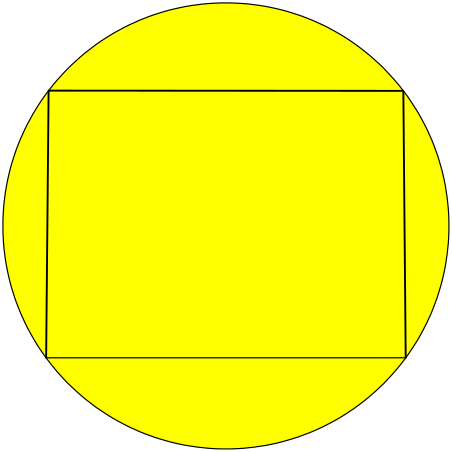
\includegraphics[ width=2.6385in, height=2.6385in,]{L4SZ270E}
	}
	
	
	\item [46.] A rectangular piece of sheet metal with and
	area of $1200 cm^{2}$ is to be bent into a cylindrical length of pipe having a volume of $600 cm^{3}$. What are the dimensions of the sheet of metal? \end{description}

\begin{description}
	\item [47.] The admission fee at an amusement park is $ \$1.50$ for children and $ \$4.00$ for adults. On a certain day, $2200$ people entered the park and the admission fees collected totalled $ \$5050$. How many children and how many adults were admitted? 
	
	\item [48.]
	A man flies a small aeroplane from Fargo to Bismarck, North Dakota - a distance of $180 \mbox{mi}$. Because he is flying into a headwind, the trip
	takes him $2$ hours. On the way back, the wind is still blowing at the same speed, so the return
	trip takes only $1$ hour and $12$ minutes. What is his speed in still air and how fast is the wind blowing? 
	
	\item [49.]
	A woman keeps fit by bicycling and running every day. One Monday she spends $\frac{1}{2} \mbox{h}$ at each activity and covers a total of $12\frac{1}{2} \mbox{mi}$. On Tuesday she runs for $12 \mbox{min}$ and cycles for $45 \mbox{min}$, covering a total of $16 \mbox{mi}$. Assuming her running and cycling speeds don't
	change from day to day, find these speeds. 
	
	\item [50.] A customer
	in a coffee shop purchases a blend of two coffees: Kenyan, costing $ \$3.50$ a pound, and Sri Lankan, costing $ \$5.60$ a pound. He buys $3 \mbox{lb}$ of the blend, which costs him $ \$11.55$. How many pounds of each kind went into the mixture?
\end{description}


\section{Some Answers}

\columnsep =30pt
\begin {multicols}{2}

\textbf{Linear Only:}

a. $\left (2 ,2\right )$ 

b. $\left (5.2 ,0.6\right )$

c. no solutions

d. no solutions

e. infinite solutions

f. $\left (-1.5 ,0\right )$\\
\break
\textbf{Mixed:}

1. $\left (3 ,1\right )$ 

3. $\left (4 ,16\right )$ 

5. $\left (2 , -2\right ) ,\left ( -2 ,2\right )$ 

7. $\left ( -25 ,5\right ) ,\left ( -25 , -5\right )$ 

9. $\left (1 ,2\right )$ 

11. $\left ( -3 ,4\right ) ,\left (3 ,4\right )$ 

13. $\left ( -2 , -1\right ) ,\left ( -2 ,1\right ) ,\left (2 , -1\right ) ,\left (2 ,1\right )$ 

17. $\left (4 ,0\right )$ 

18. $\left (0 ,0\right ) ,\left (1 ,1\right )$ 

21. $\left (6 ,2\right ) ,\left ( -2 , -6\right )$ 

25. $\left (\sqrt{5} ,2\right )\left (\sqrt{5} , -2\right )$ 

31. $\left ( -0.33 ,5.33\right )$ 

35. $\left ( -4.51 ,2.17\right ) ,\left (4.91 , -0.97\right )$ 

37. $\left (1.23 ,3.87\right ) ,\left ( -0.35 , -4.21\right )$ \\
\break
\textbf{Word Problems}\\

41. $12 \mbox{cm}$ by $15 \mbox{cm}$ 

42. $7 \mbox{ft}$ and $24 \mbox{ft}$ 

44. $4 \sqrt{5} \mbox{in}$ by $8 \sqrt{5} \mbox{in}$ 

46. The dimensions of the sheet are $2 \pi $ by $\frac{600}{\pi }$  

47. The number of children admitted was 1500 and the number
of adults was 700. 

48. Plane's speed $120 mi/\mbox{h}$, wind speed $30 mi/\mbox{h}$ 

49. Run $5 mi/\mbox{h}$, cycle $20 mi/\mbox{h}$ 

50. $2.5$ pounds of Kenyan coffee and $0.5$ pounds of Sri Lankan coffee should be mixed. 



\end {multicols}

\columnsep =30pt
\begin {multicols}{2}

\end {multicols}

